\documentclass[12pt]{article} % use larger type; default would be 10pt
\usepackage[utf8]{inputenc} % set input encoding (not needed with XeLaTeX)

%%% PAGE DIMENSIONS
\usepackage{geometry} % to change the page dimensions
\geometry{a4paper} % or letterpaper (US) or a5paper or....
\geometry{margin=2cm} % or letterpaper (US) or a5paper or....

\usepackage{graphicx} % support the \includegraphics command and options
\usepackage[parfill]{parskip} % Activate to begin paragraphs with an empty line rather than an indent
\usepackage{times} % for Times Roman default font

%%% PACKAGES
\usepackage{booktabs} % for much better looking tables
\usepackage{array} % for better arrays (eg matrices) in maths
\usepackage{paralist} % very flexible & customisable lists (eg. enumerate/itemize, etc.)
\usepackage{verbatim} % adds environment for commenting out blocks of text & for better verbatim
\usepackage{subfig} % make it possible to include more than one captioned figure/table in a single float
\usepackage{caption}
\usepackage{hyperref}

%%% HEADERS & FOOTERS
\usepackage{fancyhdr} % This should be set AFTER setting up the page geometry
\pagestyle{fancy} % options: empty , plain , fancy
\renewcommand{\headrulewidth}{0pt} % customise the layout...
\lhead{}\chead{}\rhead{}
\lfoot{}\cfoot{\thepage}\rfoot{}

\makeatletter
\renewcommand{\maketitle}{%
  {\bfseries{\scshape{\Large{\@title\par}}}}
}
\makeatother

\hyphenation{Kiwi-bank} % otherwise it may get hyphenated as Ki-wibank

%%% END Article customizations

%%% The "real" document content comes below...

\title{Lucretia Biv Report: 23-24 November 2019}

\begin{document}
  \maketitle

\section{Background}

DoC have sought community support to maintain a number of huts/bivs in the Lewis Pass area, including Lucretia Biv and Lake Man Biv.  We have already attended to \href{https://drive.google.com/open?id=1DdW8LlDO5h38anP1OH9vCVlA9F1gLeeN}{Lake Man Biv}.  This document reports on a visit to Lucretia Biv on 23-24 November 2019.  The purpose of the visit was to assess the state of the Biv and determine whether or not we would be interested/capable of taking on its maintenance.

\section{Current state}

Lucretia Biv is a basic two-bunk biv, similar to Lake Man Biv but with a fire place (Figure \ref{LB01}).  The Biv is basically sound, but leakage around the fireplace has caused some internal damage.  Furthermore, the fireplace provides an entry point for rodents.  However, the sub-floor seems in good condition, although there is a bearer which requires a pile (Figure \ref{LB02}).  The roof has lead-head nails and lead-edged ridge flashing.

\begin{figure}[ht]
%\centering
\begin{minipage}{.5\linewidth}
\begin{center}
  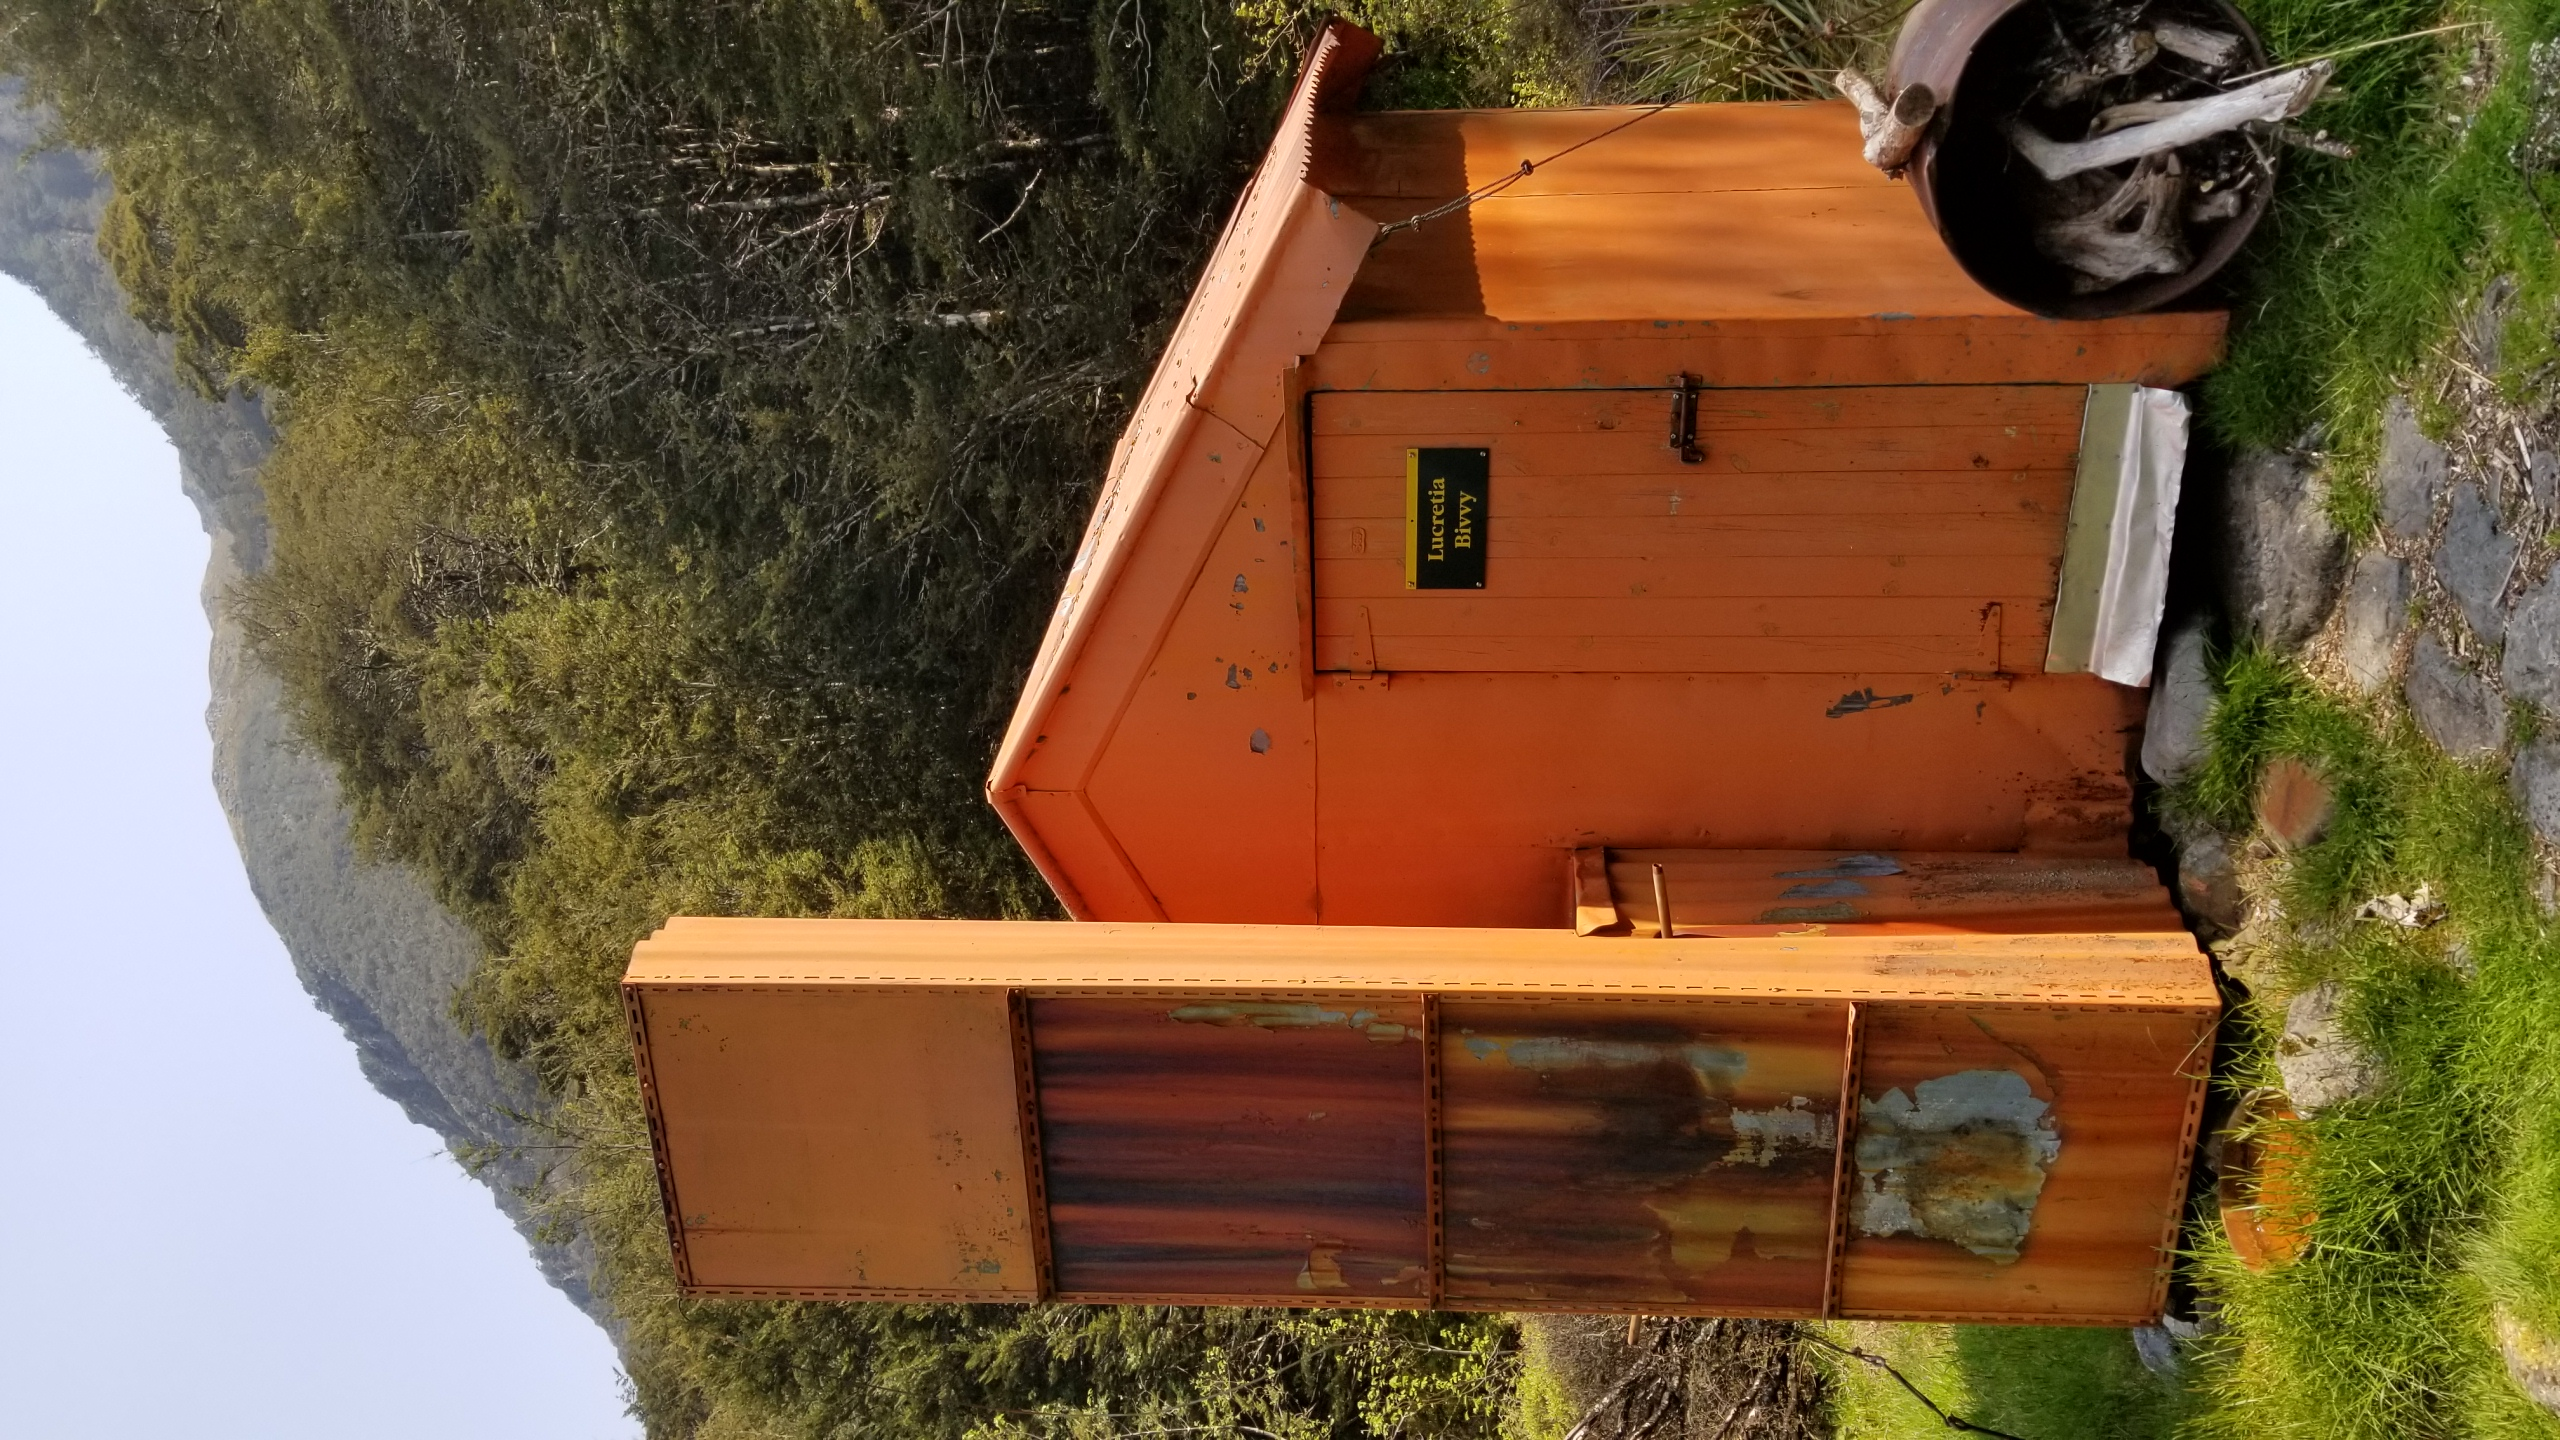
\includegraphics[width=8cm, angle=270]{LucretiaBivReport23Nov2019Photo1}
  \caption{Lucretia Biv}
  \label{LB01}
\end{center}
\end{minipage}
\begin{minipage}{.5\linewidth}
\begin{center}
  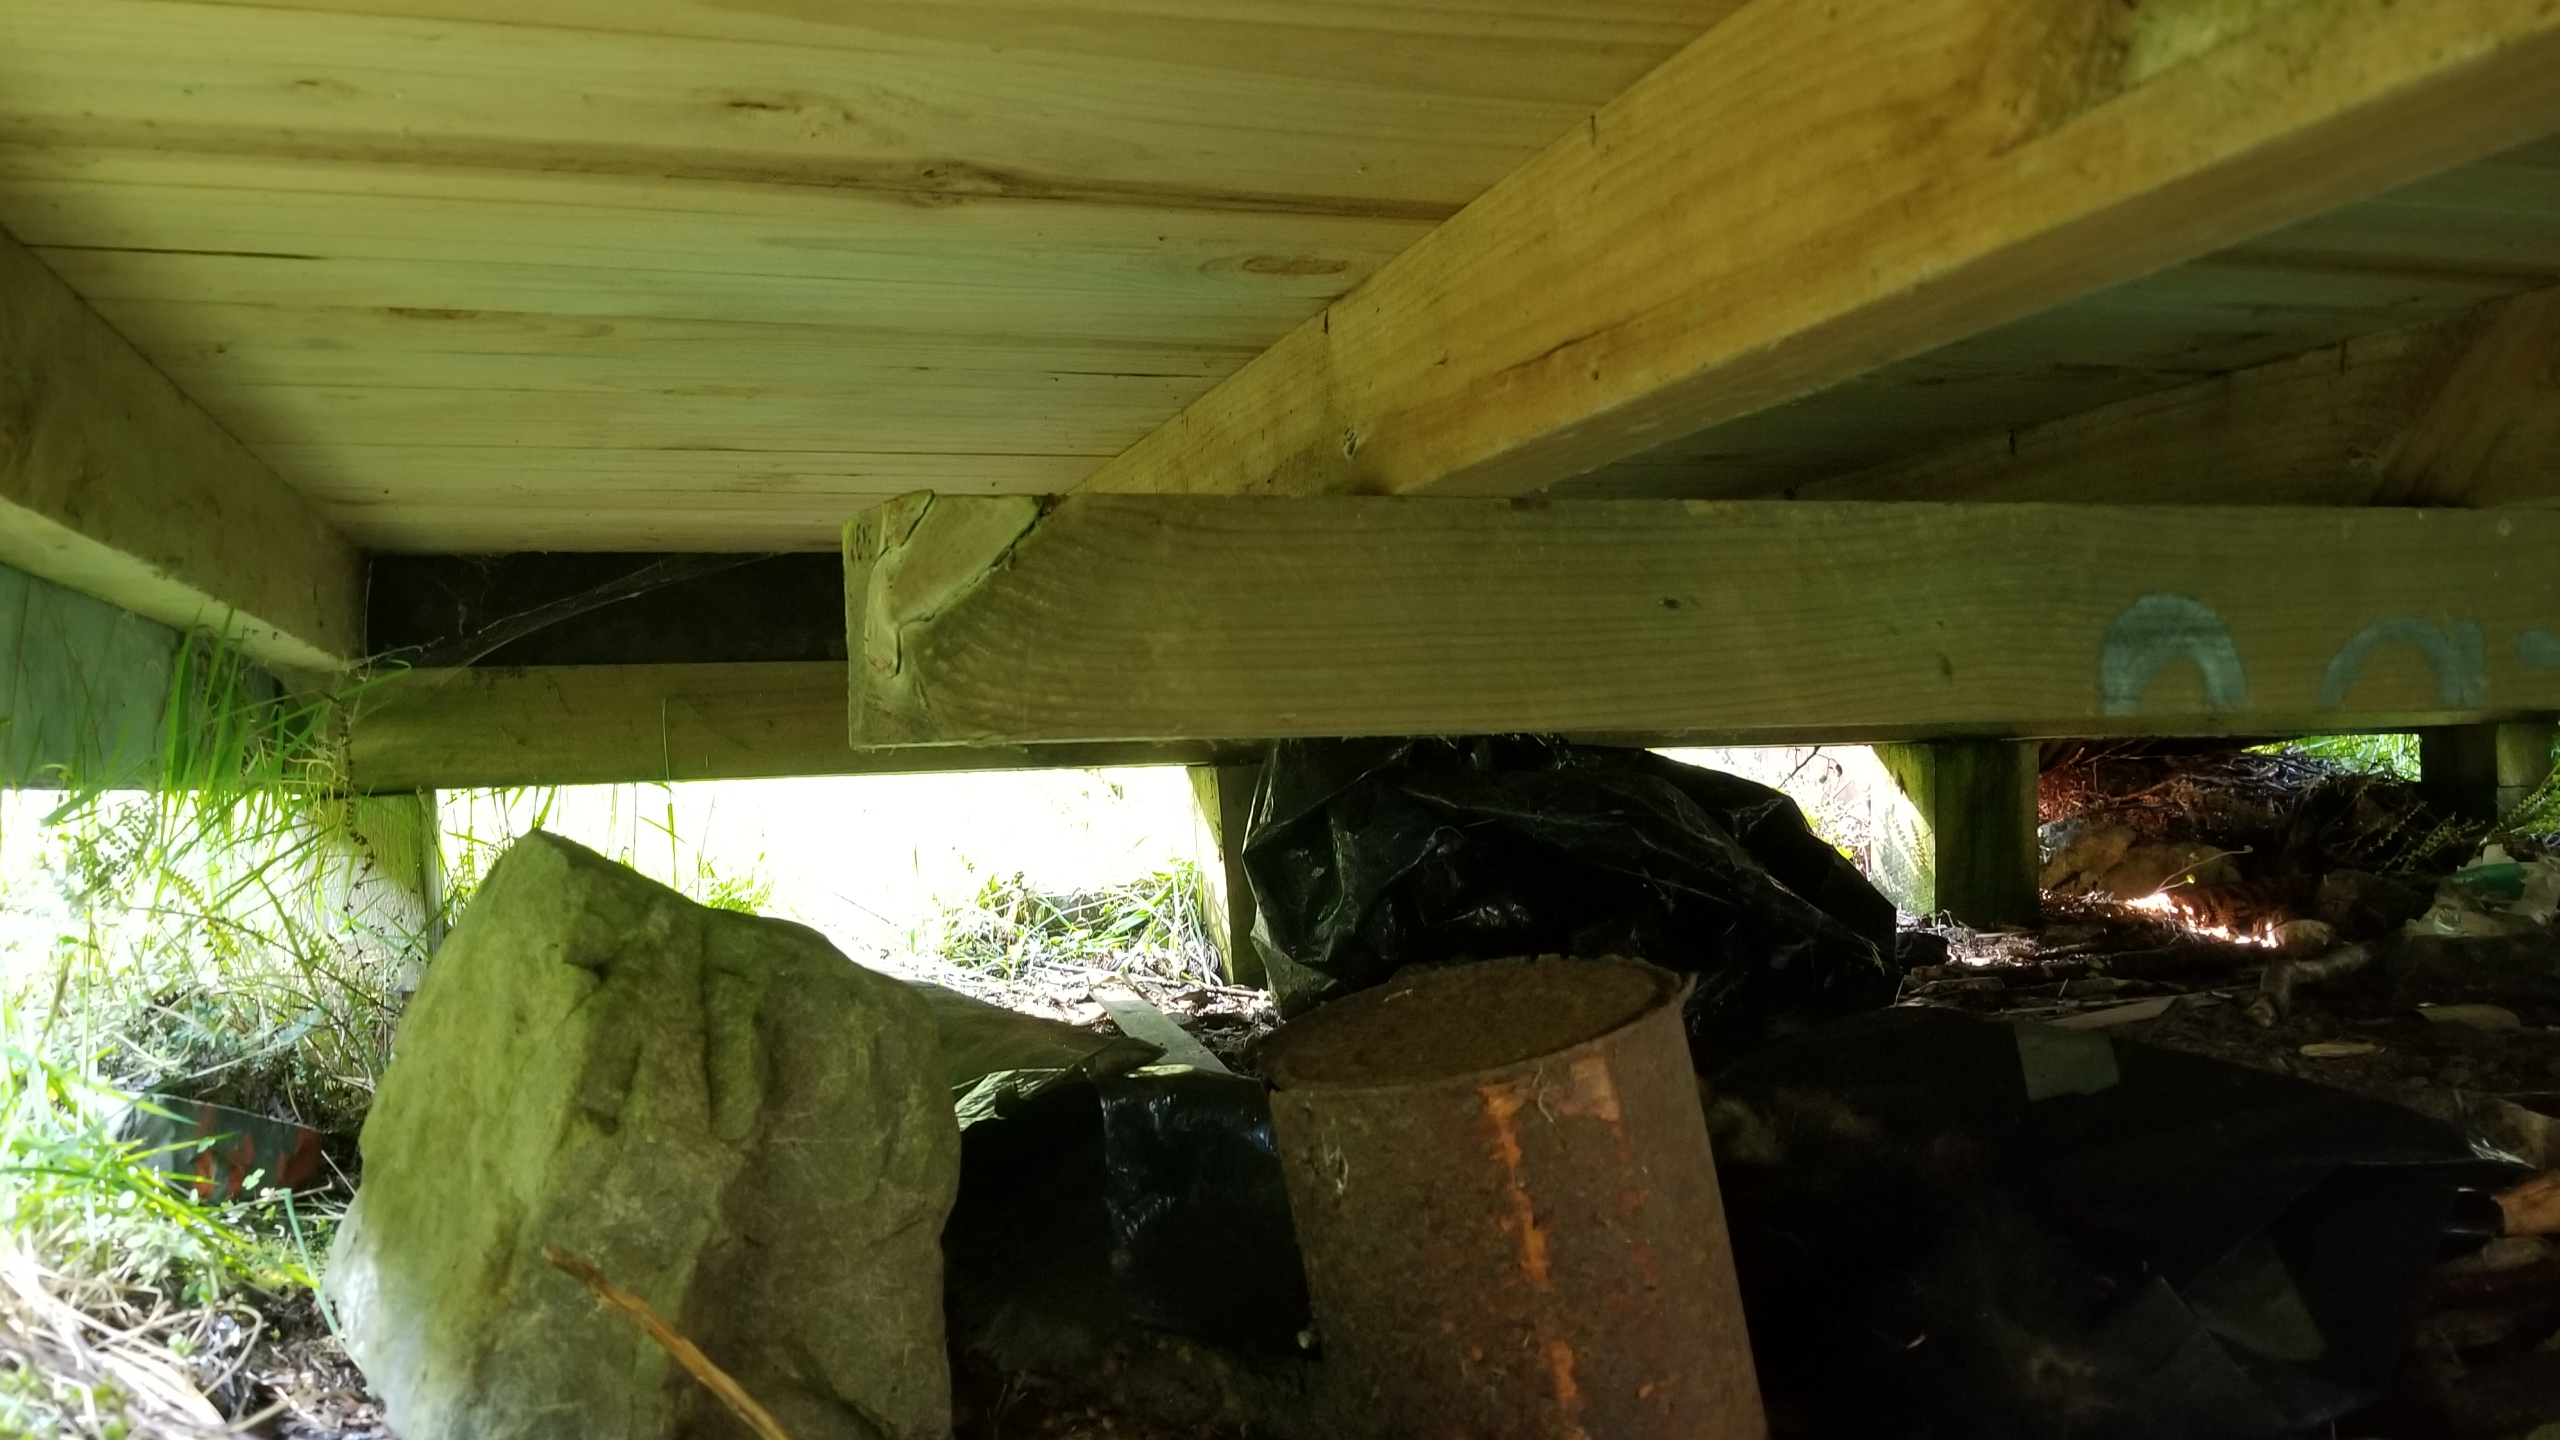
\includegraphics[width=8cm]{LucretiaBivReport23Nov2019Photo2}
  \caption{Underfloor showing `hanging' bearer}
  \label{LB02}
\end{center}
\end{minipage}
\end{figure}

\section{Maintenance and improvements}

\subsection{Required}

\begin{itemize}
 \item Repair fireplace and replace the chimney (Figures \ref{LB03} and \ref{LB04}).  This will require some concrete work on the base, a new iron fire backing\footnote{During an earlier visit (May 2017) we noticed that the fire smoked badly unless the window or door was open.  Also, most of the heat went up the chimney.   Heat exchange pipes connected to the outside should alleviate both of these problems}, and a slightly redesigned chimney with a weather cap and additional flashing (as done at \href{https://www.backcountrytrust.org.nz/projects-blog/how-to-renovate-a-nzfs-2-bunk-biv}{Mackenzie Biv})
 \item Build a two-bay woodshed.  There is ample firewood around the hut, but inadequate storage
 \item Replace the iron on the roof.  Arguably it would be satisfactory to simply replace the lead-head nails with hex-screws (there are about 90), and paint the existing roof.  However, if the iron is replaced, the old iron could be used to build the woodshed, and proper flashing could be used for the ridge and gable ends
 \item Paint the exterior.  The paint appears to be in better condition than that of Lake Man Biv was.  Thus, it may be that spot priming and a couple of top coats will be sufficient (although it is advisable to go prepared for a full prime and some rust treatment)
 \item Prior to painting there are a few small nail holes in the cladding which will need filling
 \item Clear grass and other vegetation from around the biv to allow good air-flow under it
 \item Fit a weather ledge on the door to prevent water creeping under it during driving rain
 \item Regrettably, there is quite a lot of accumulated rubbish both under and about the biv.  This should be removed (or, perhaps, buried)
 \item Replace canvas on the bunks with slats.  There are new mattresses in the biv but the bunks are slightly to narrow for them.  Thus, the bunks should be made slightly wider at the same time
 \item Install small stainless steel cooking bench (Figure \ref{LB06})
 \item Replace a couple of sections of flooring near the fireplace.  These have begun to rot due to the water leakage from the chimney (Figure \ref{LB05})
 \item Replace a section of internal wall lining which is rotting (also due to leakage from the chimney)
 \item Install pile under the `hanging' bearer (Figure \ref{LB02})
\end{itemize}
 
\begin{figure}[ht]
%\centering
\begin{minipage}{.5\linewidth}
\begin{center}
   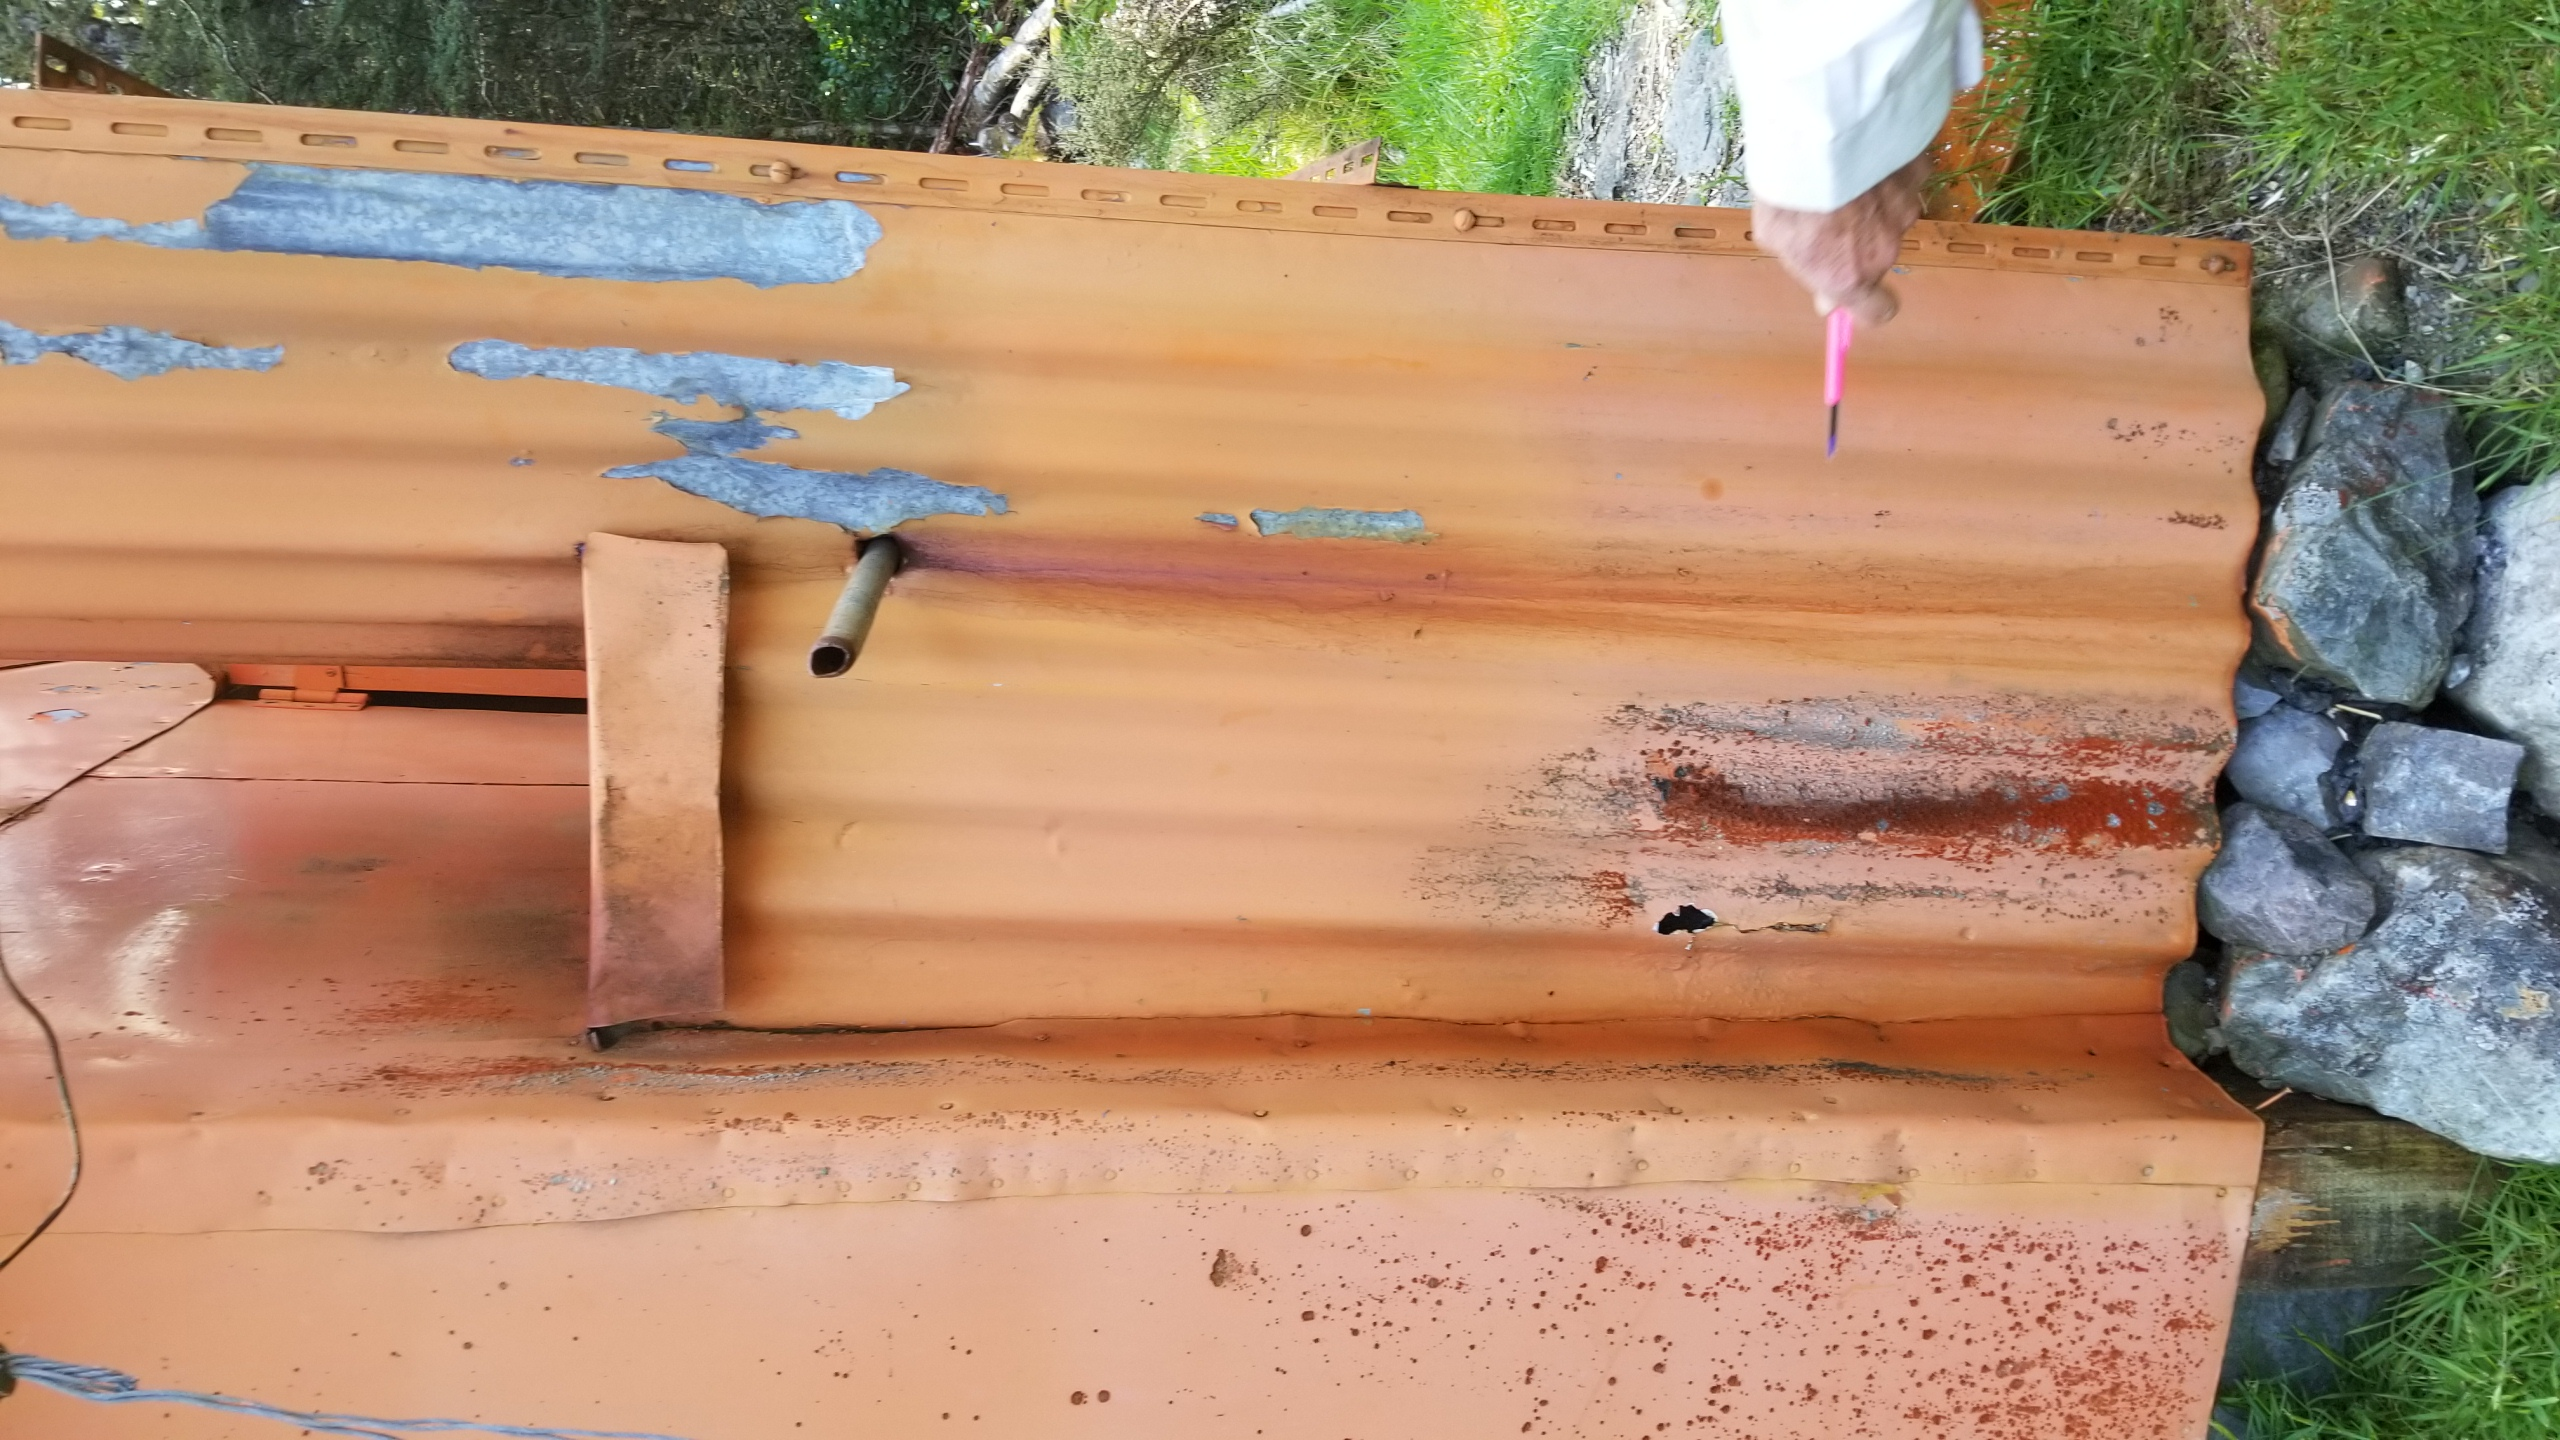
\includegraphics[width=8cm, angle=270]{LucretiaBivReport23Nov2019Photo3}
   \caption{Chimney showing deteriorated iron}
   \label{LB03}
\end{center}
\end{minipage}
\begin{minipage}{.5\linewidth}
\begin{center}
   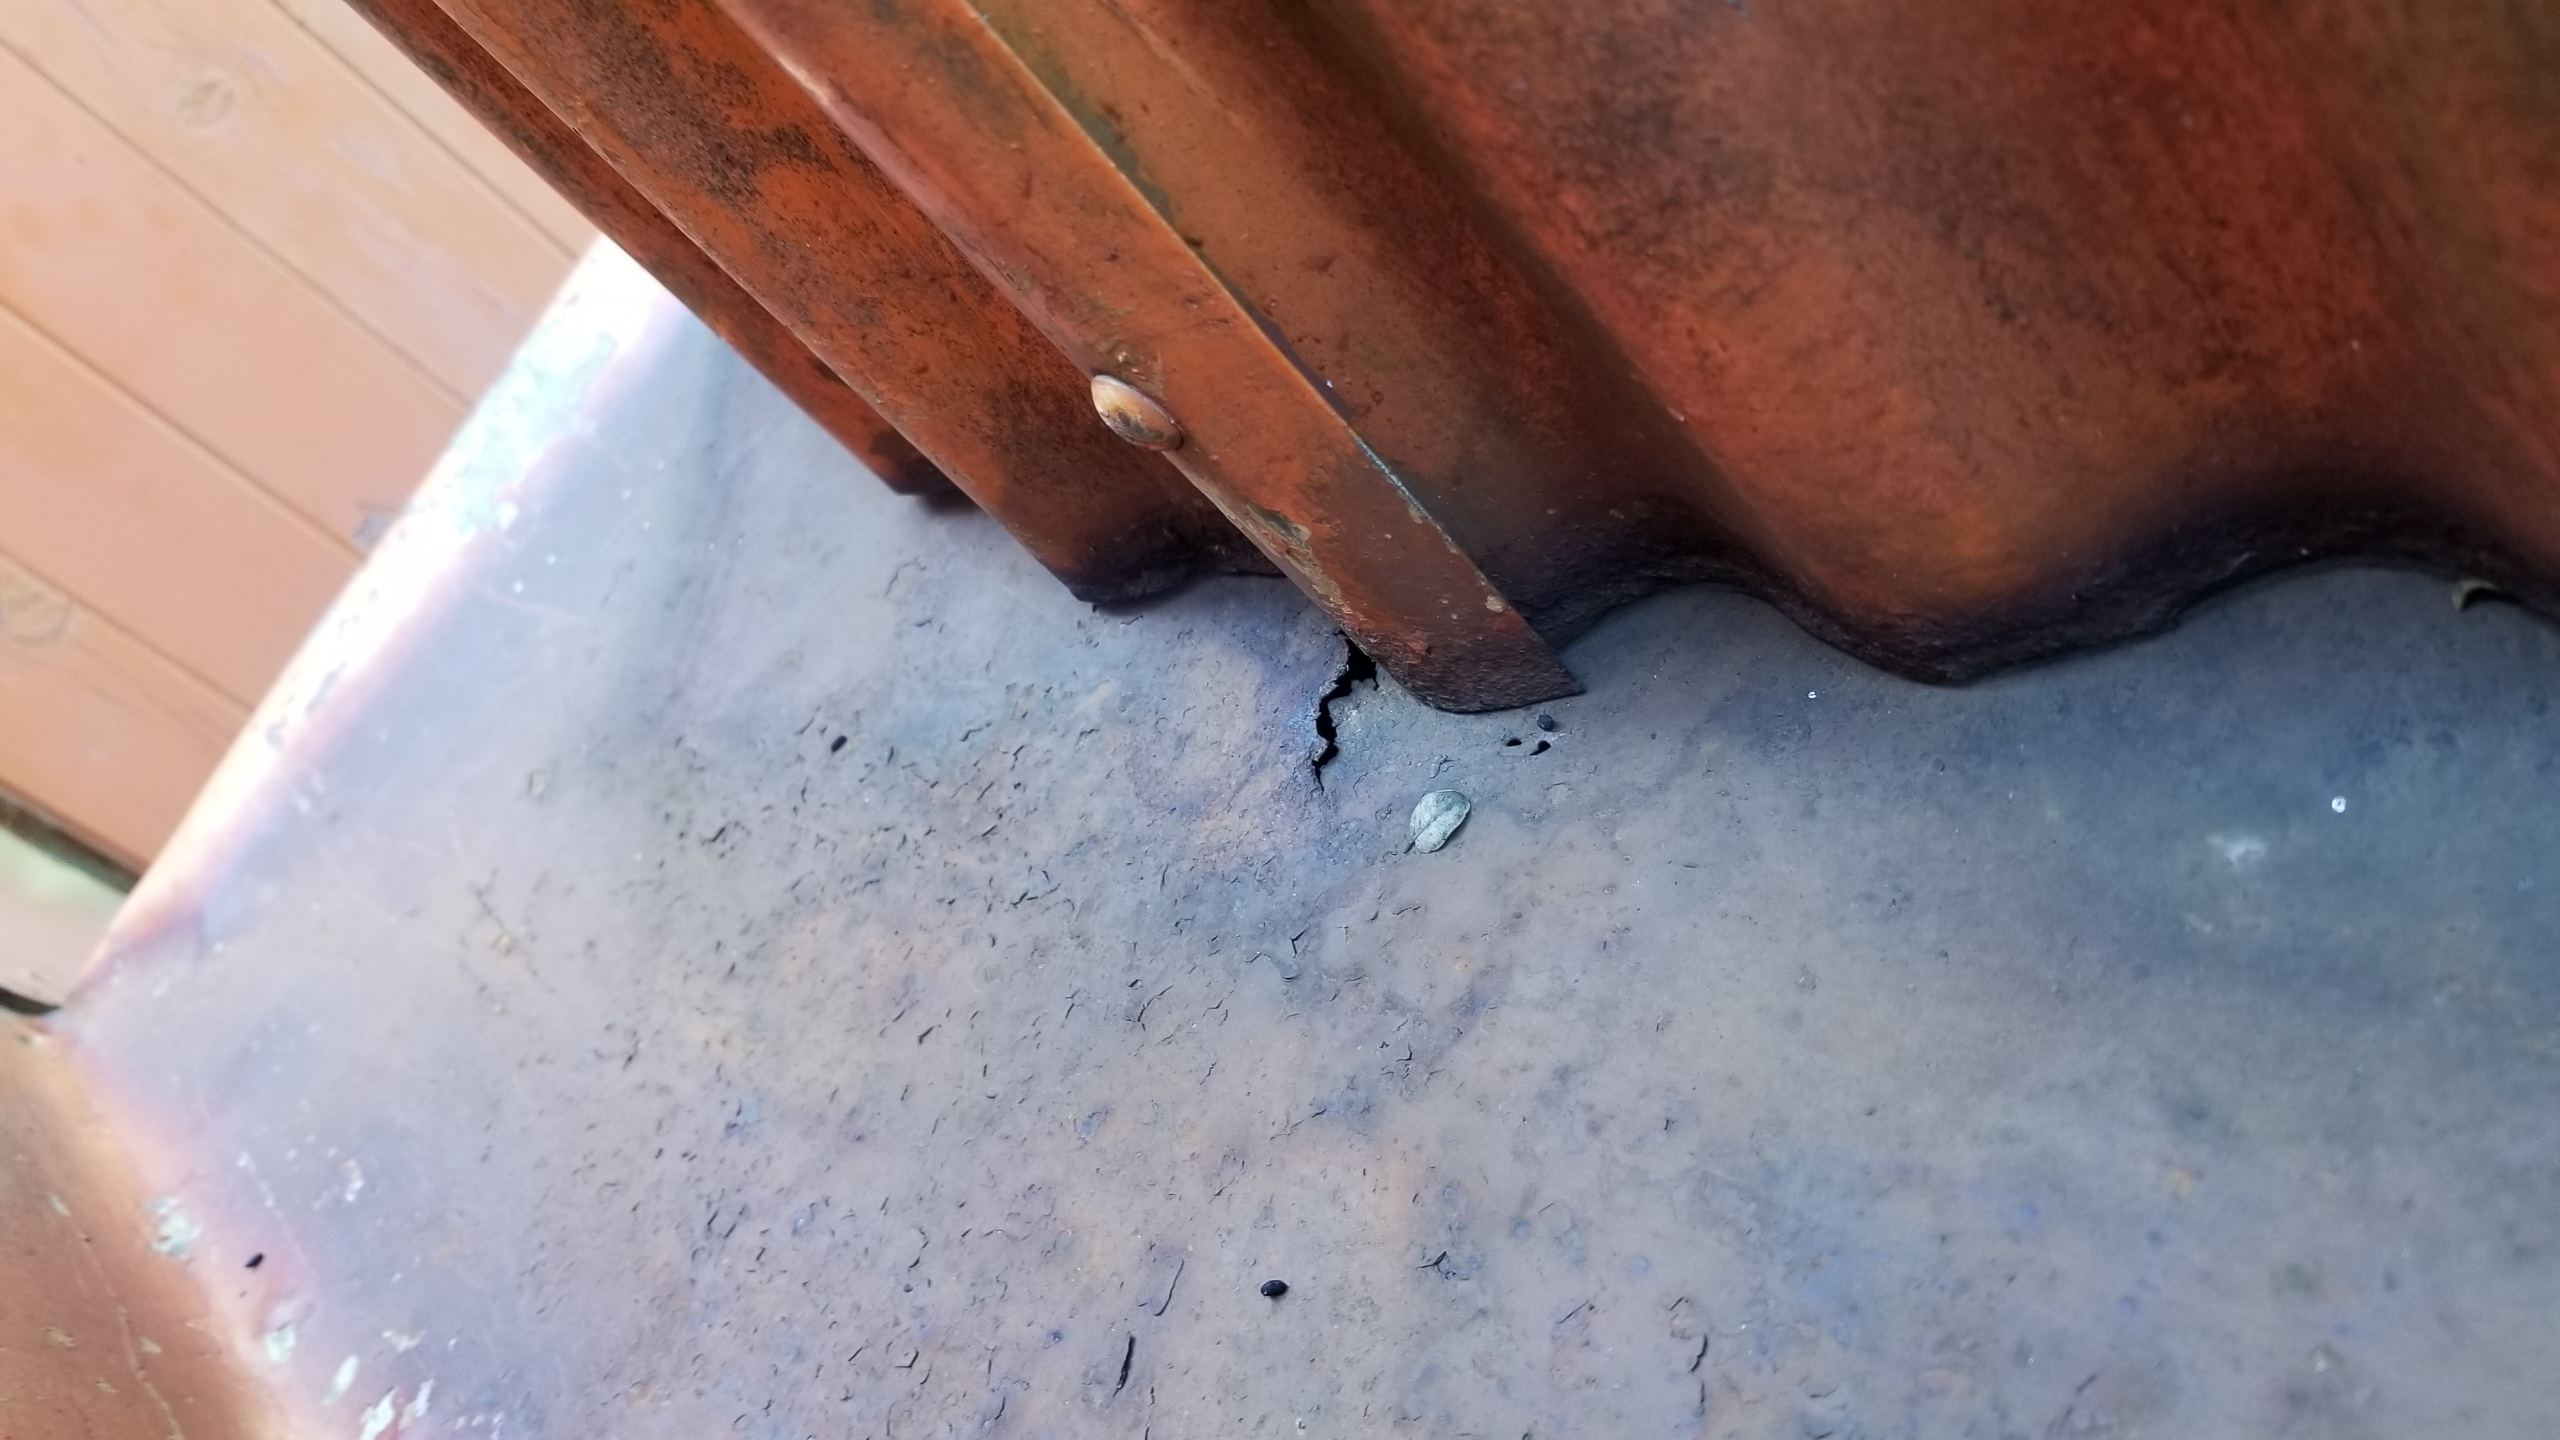
\includegraphics[width=8cm]{LucretiaBivReport23Nov2019Photo4}
   \caption{Rust and hole in flat section on the chimney}
   \label{LB04}
\end{center}
\end{minipage}
\end{figure}

\begin{figure}[ht]
%\centering
\begin{minipage}{.5\linewidth}
\begin{flushleft}
   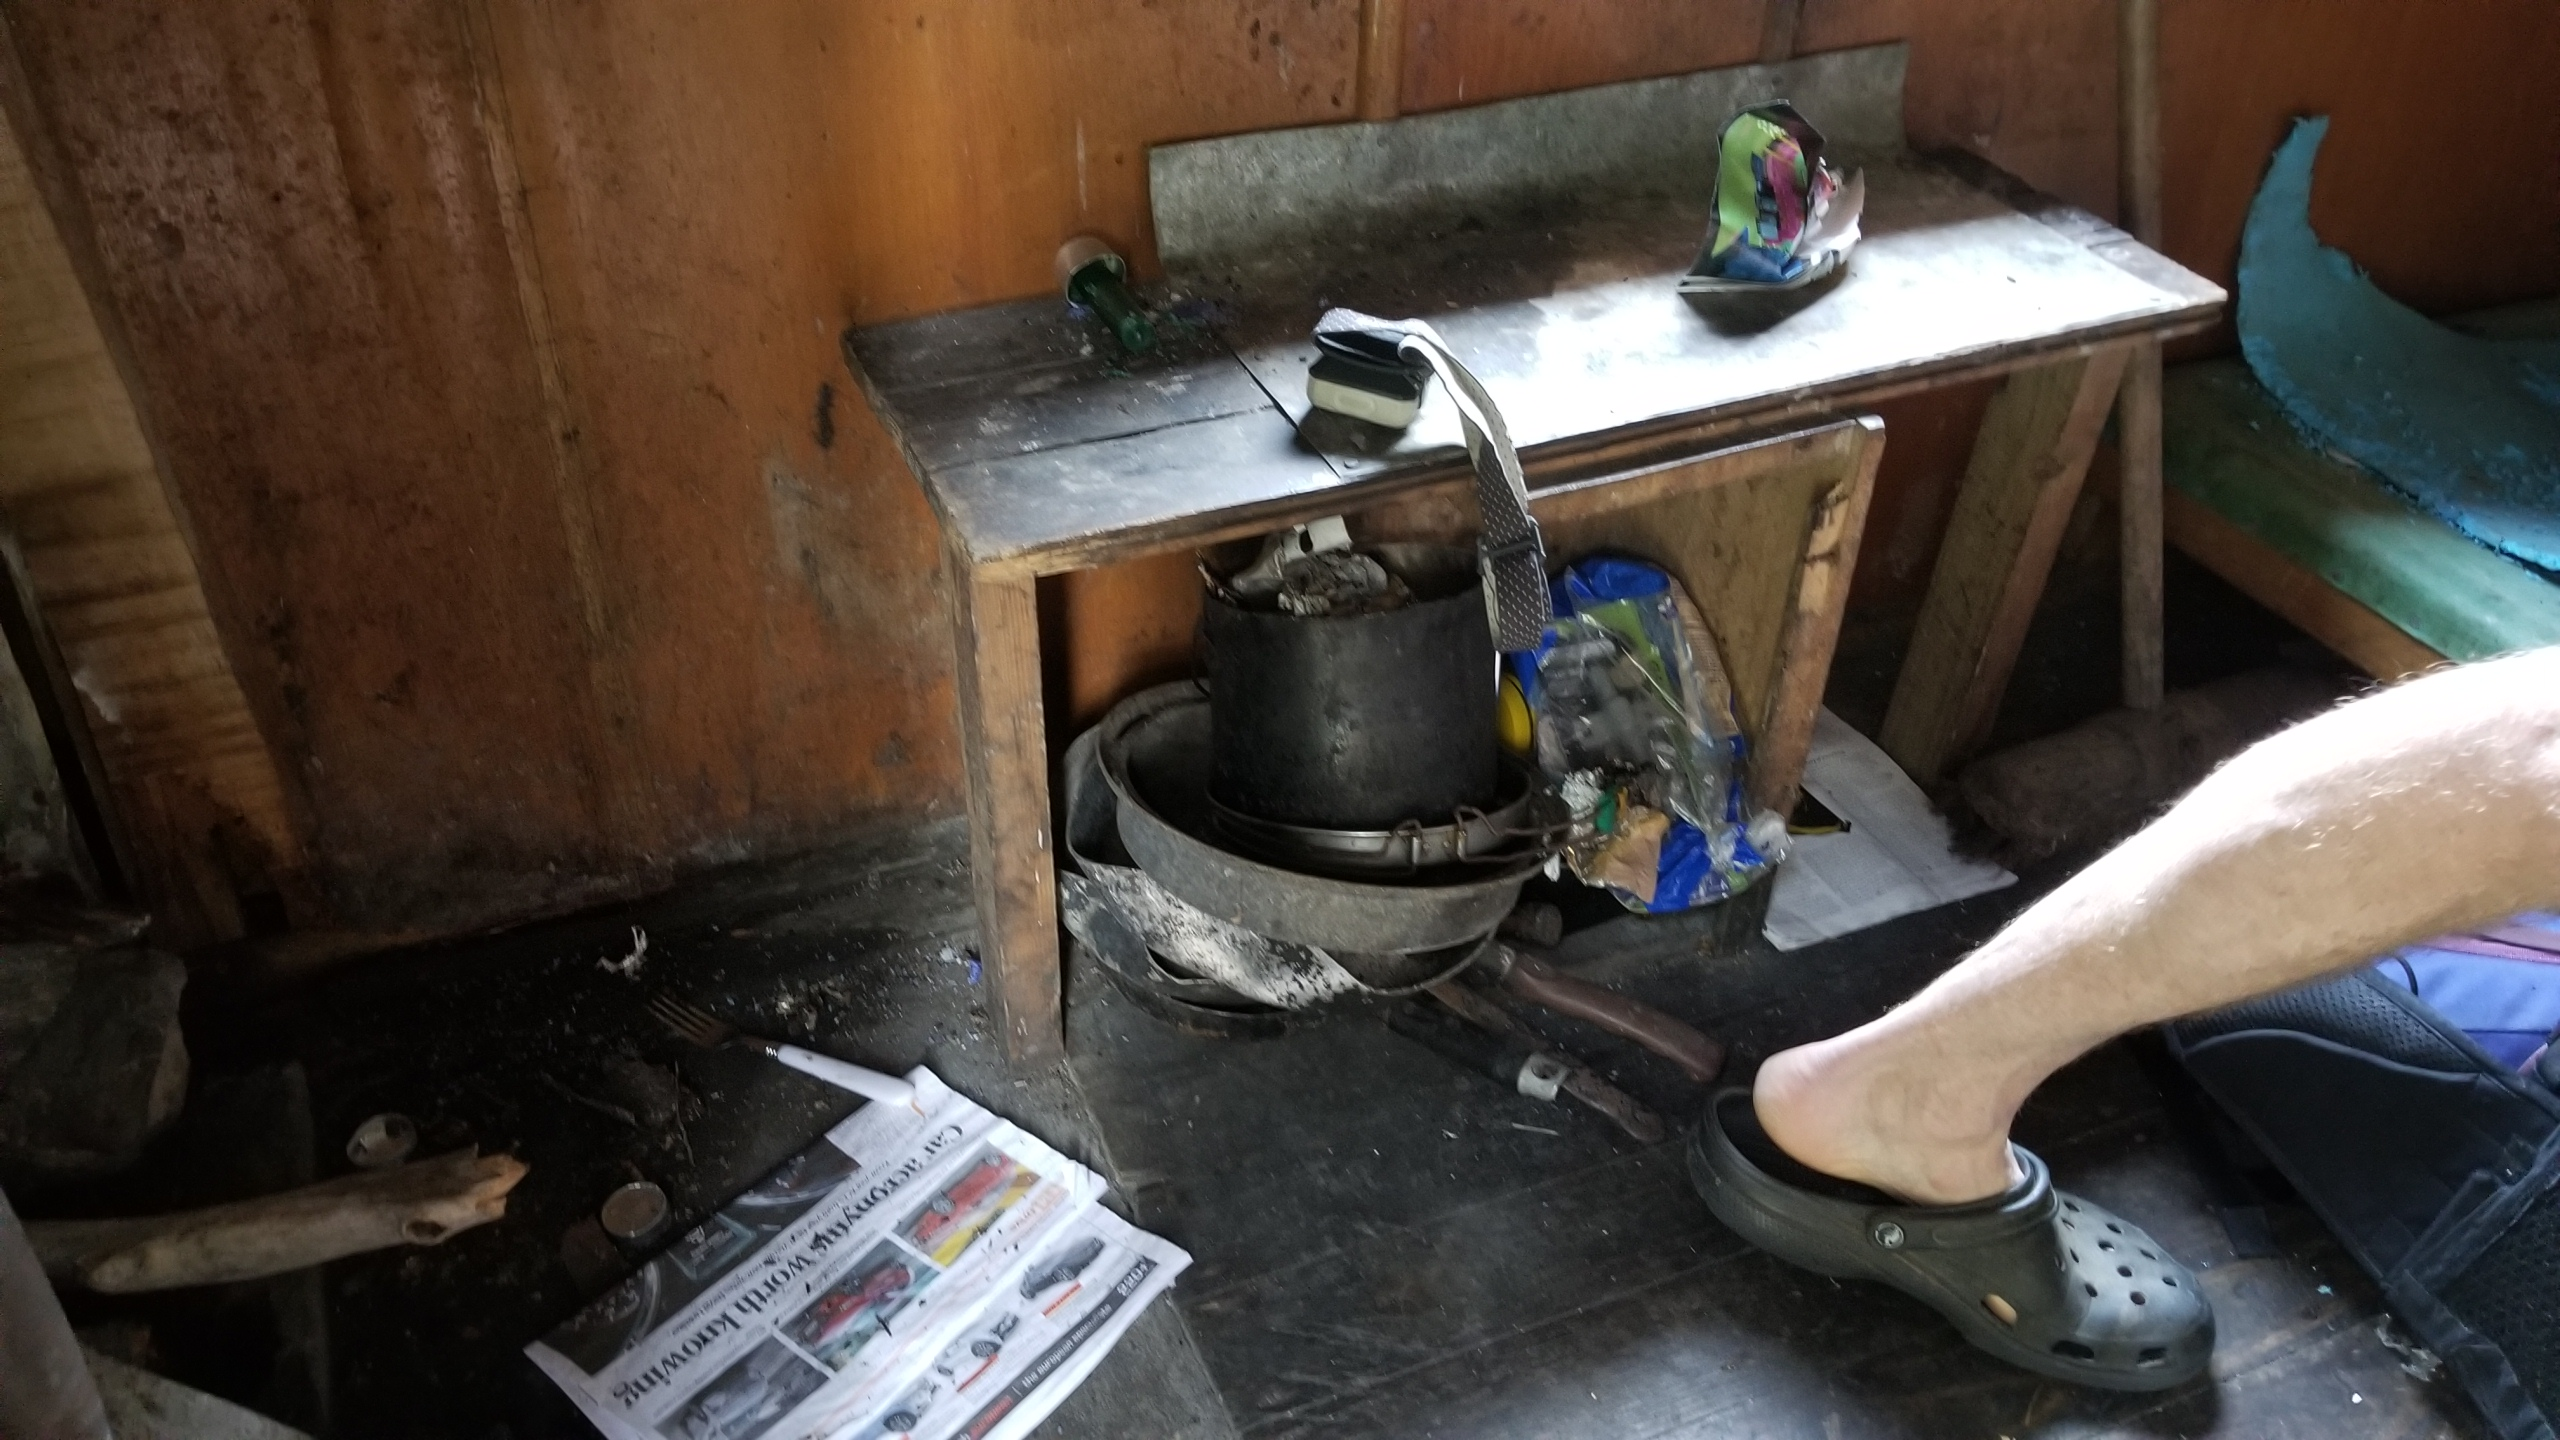
\includegraphics[width=8cm]{LucretiaBivReport23Nov2019Photo6}
   \caption{Current cooking bench}
   \label{LB06}
\end{flushleft}
\end{minipage}
\begin{minipage}{.5\linewidth}
\begin{center}
   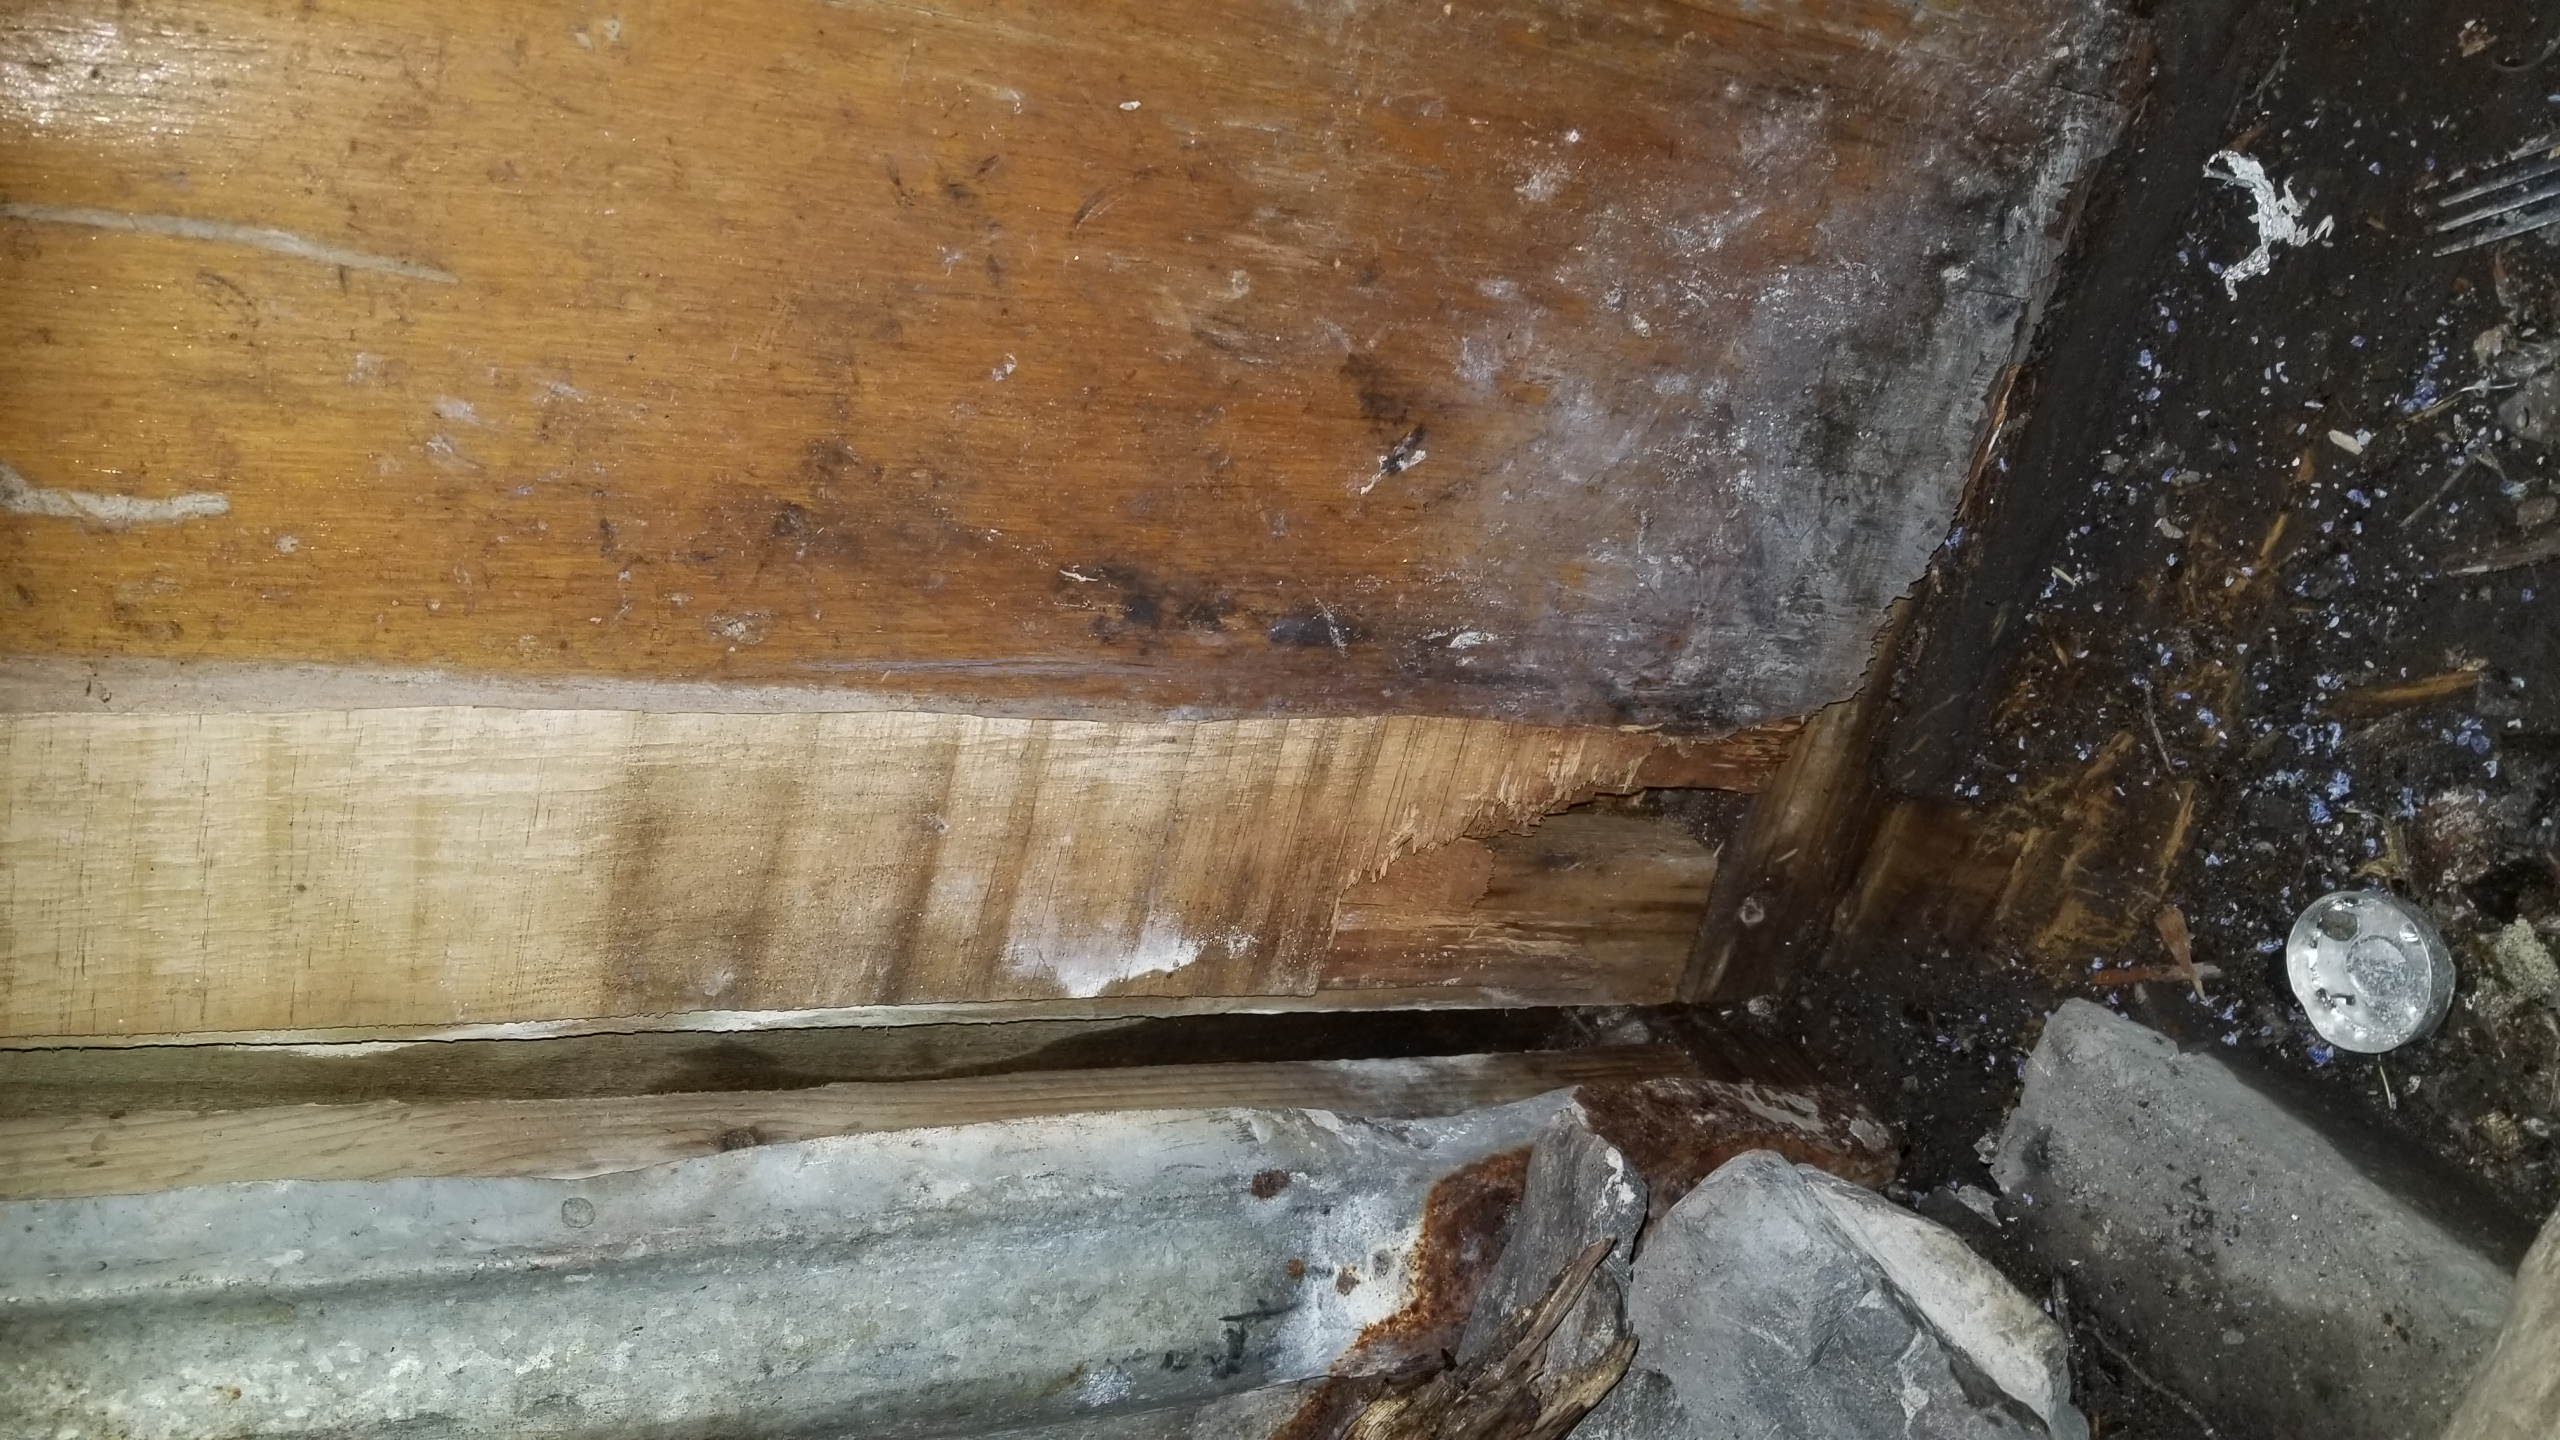
\includegraphics[width=8cm, angle=270]{LucretiaBivReport23Nov2019Photo5}
   \caption{Wet and deteriorating floor boards and wall lining next to the fireplace}
   \label{LB05}
\end{center}
\end{minipage}
\end{figure}

\subsection{Desirable}

\begin{itemize}
 \item As mentioned, the roof needs attention.  Thus, one might as well remove the purlins, and install a ceiling lining (plywood painted white) and some insulation
 \item Internal trim around the doorway to reduce unwanted draft
 \item Better method of securing the door from the inside (i.e., an internal door bolt)
 \item The view of the waterfall from the doorway is magnificent (Figure \ref{LB08}), thus it would be nice to have a window in this door.  That would also provide more light in the biv which is somewhat dark
  \item Rebuild shelves above the mantel-piece (which is currently missing)
  \item Install a tilting seat similar to that at \href{https://drive.google.com/open?id=1DdW8LlDO5h38anP1OH9vCVlA9F1gLeeN}{Lake Man Biv}
  \item Put extra markers on the track into the hut and trim some of the vegetation.  This would depend on there being sufficient people-power when the renovations are undertaken

\end{itemize}

\begin{figure}[ht]
%\centering
\begin{minipage}{.5\linewidth}
\begin{flushleft}
   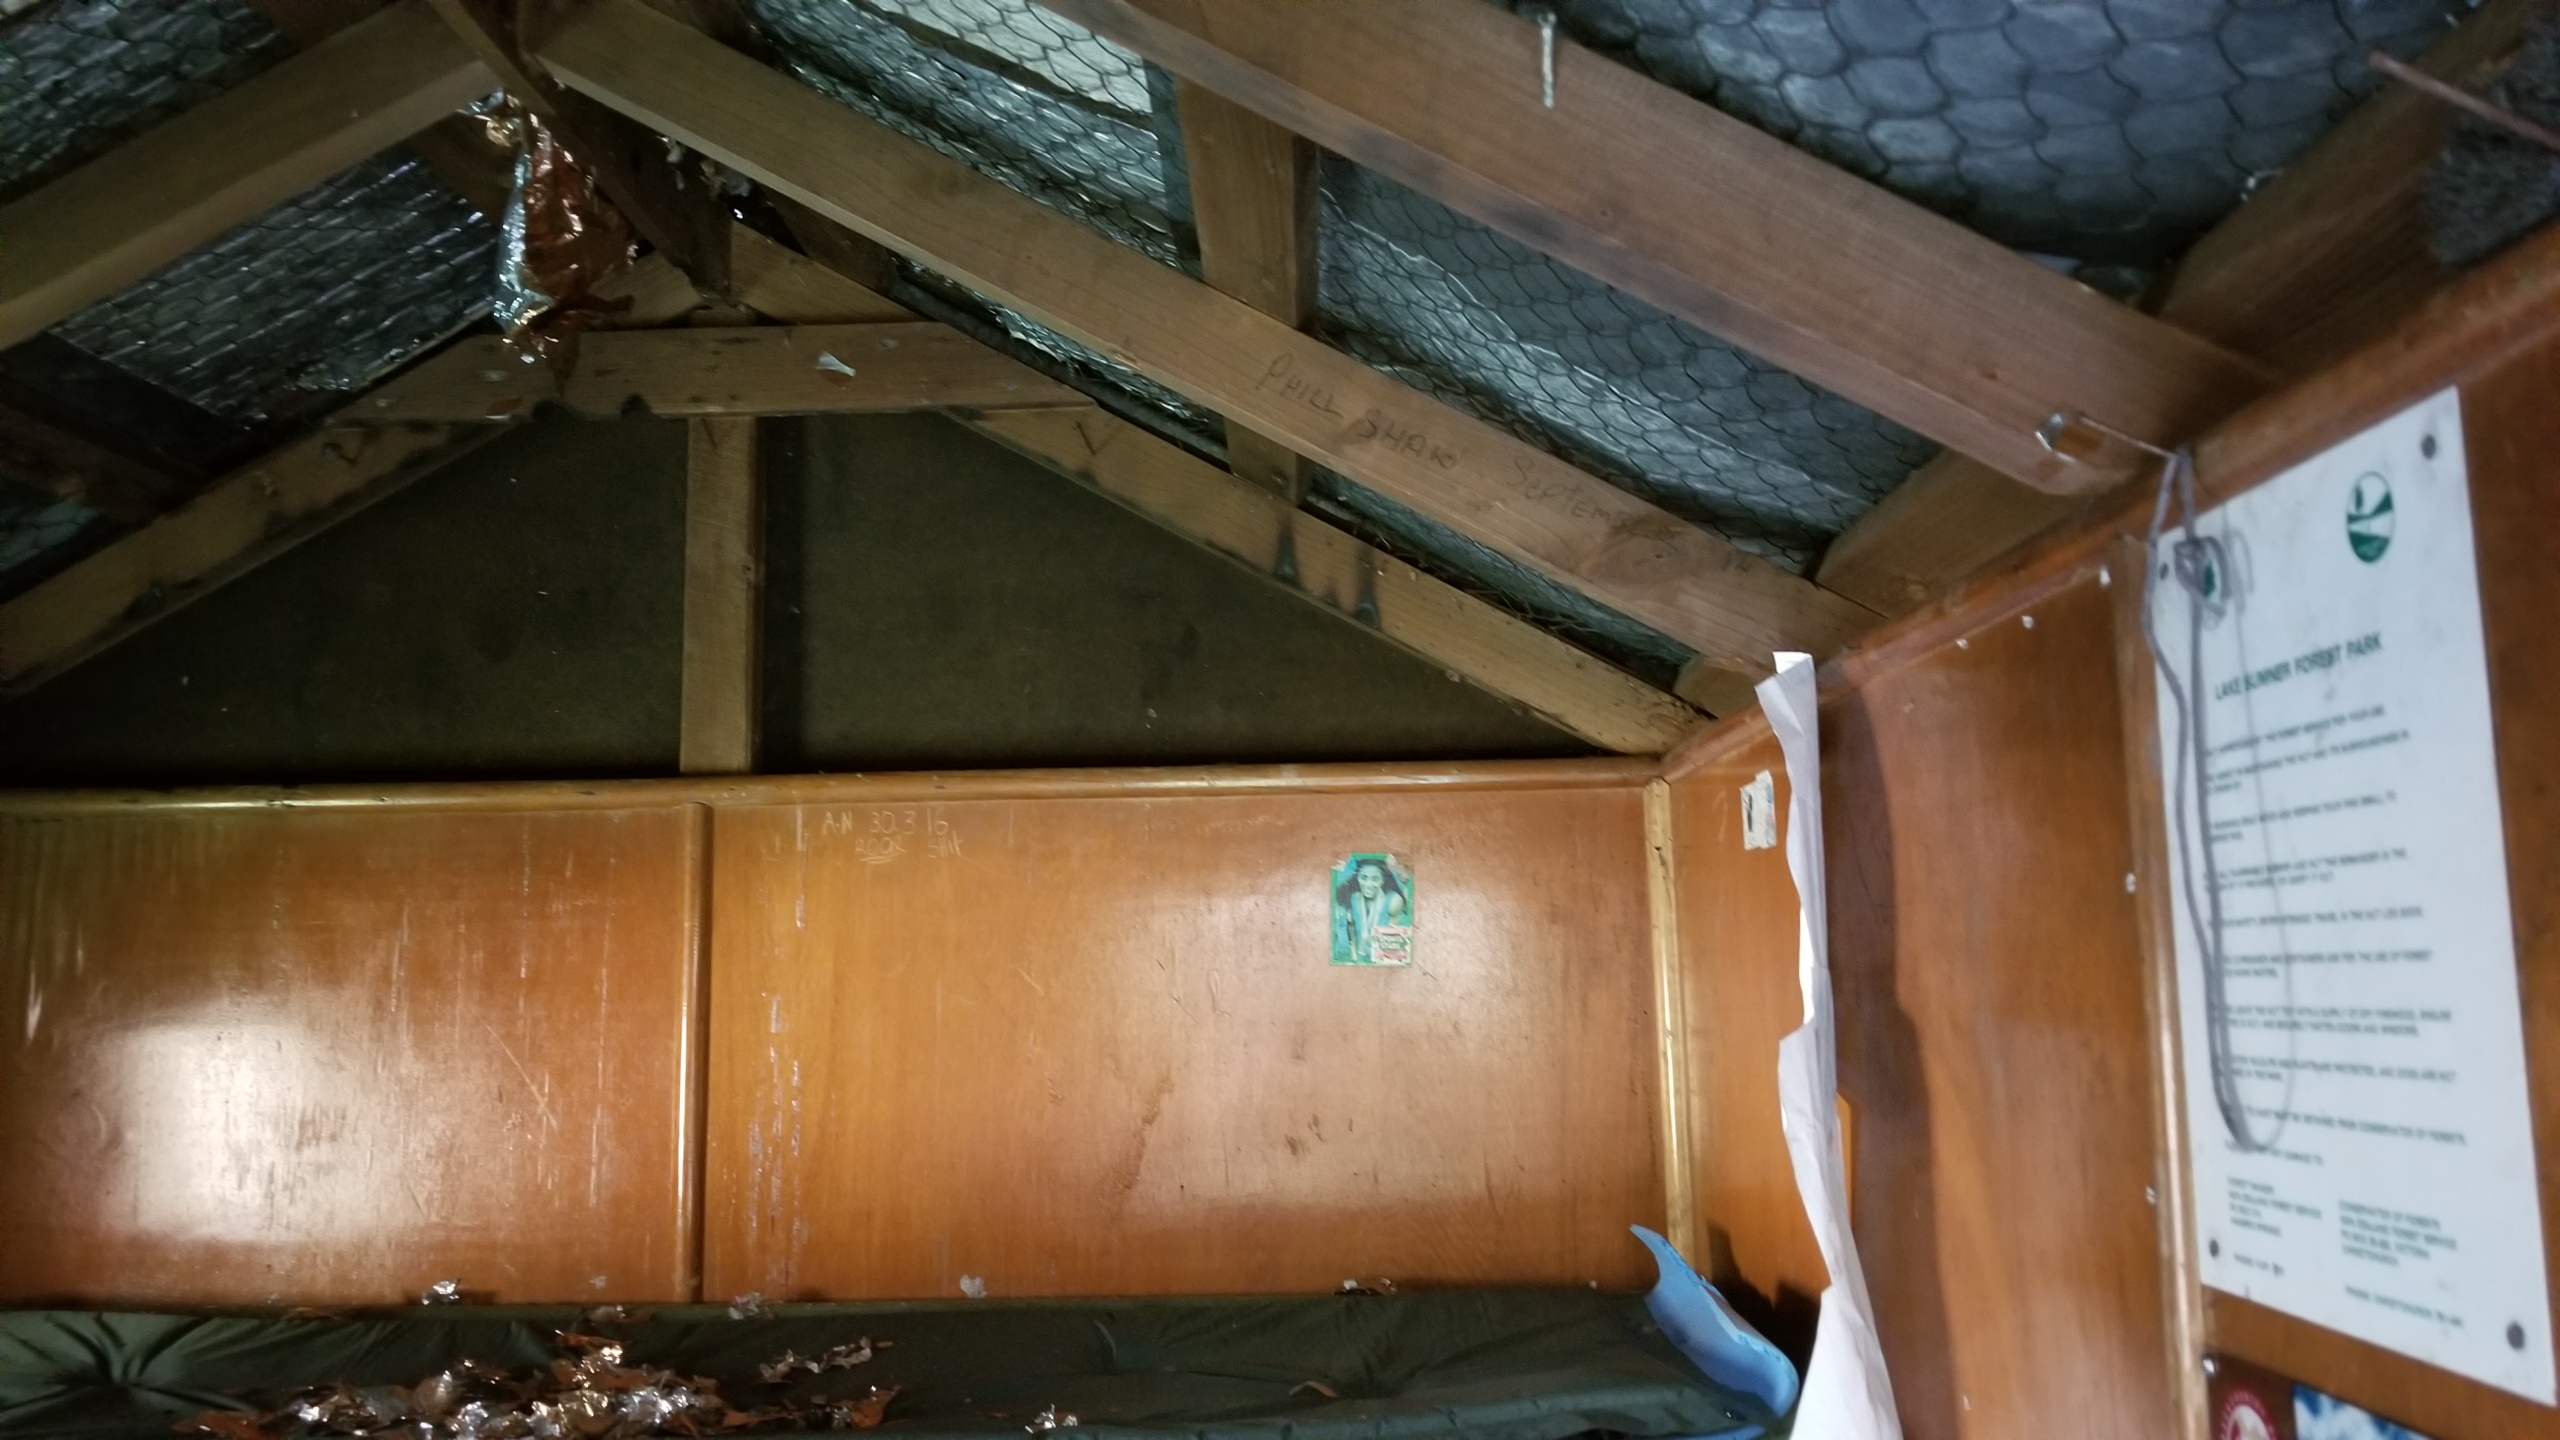
\includegraphics[width=8cm]{LucretiaBivReport23Nov2019Photo7}
   \caption{Interior of biv (with light from the open door).  Note the vermin chewings on the top bunk}
   \label{LB07}
\end{flushleft}
\end{minipage}
\begin{minipage}{.5\linewidth}
\begin{center}
   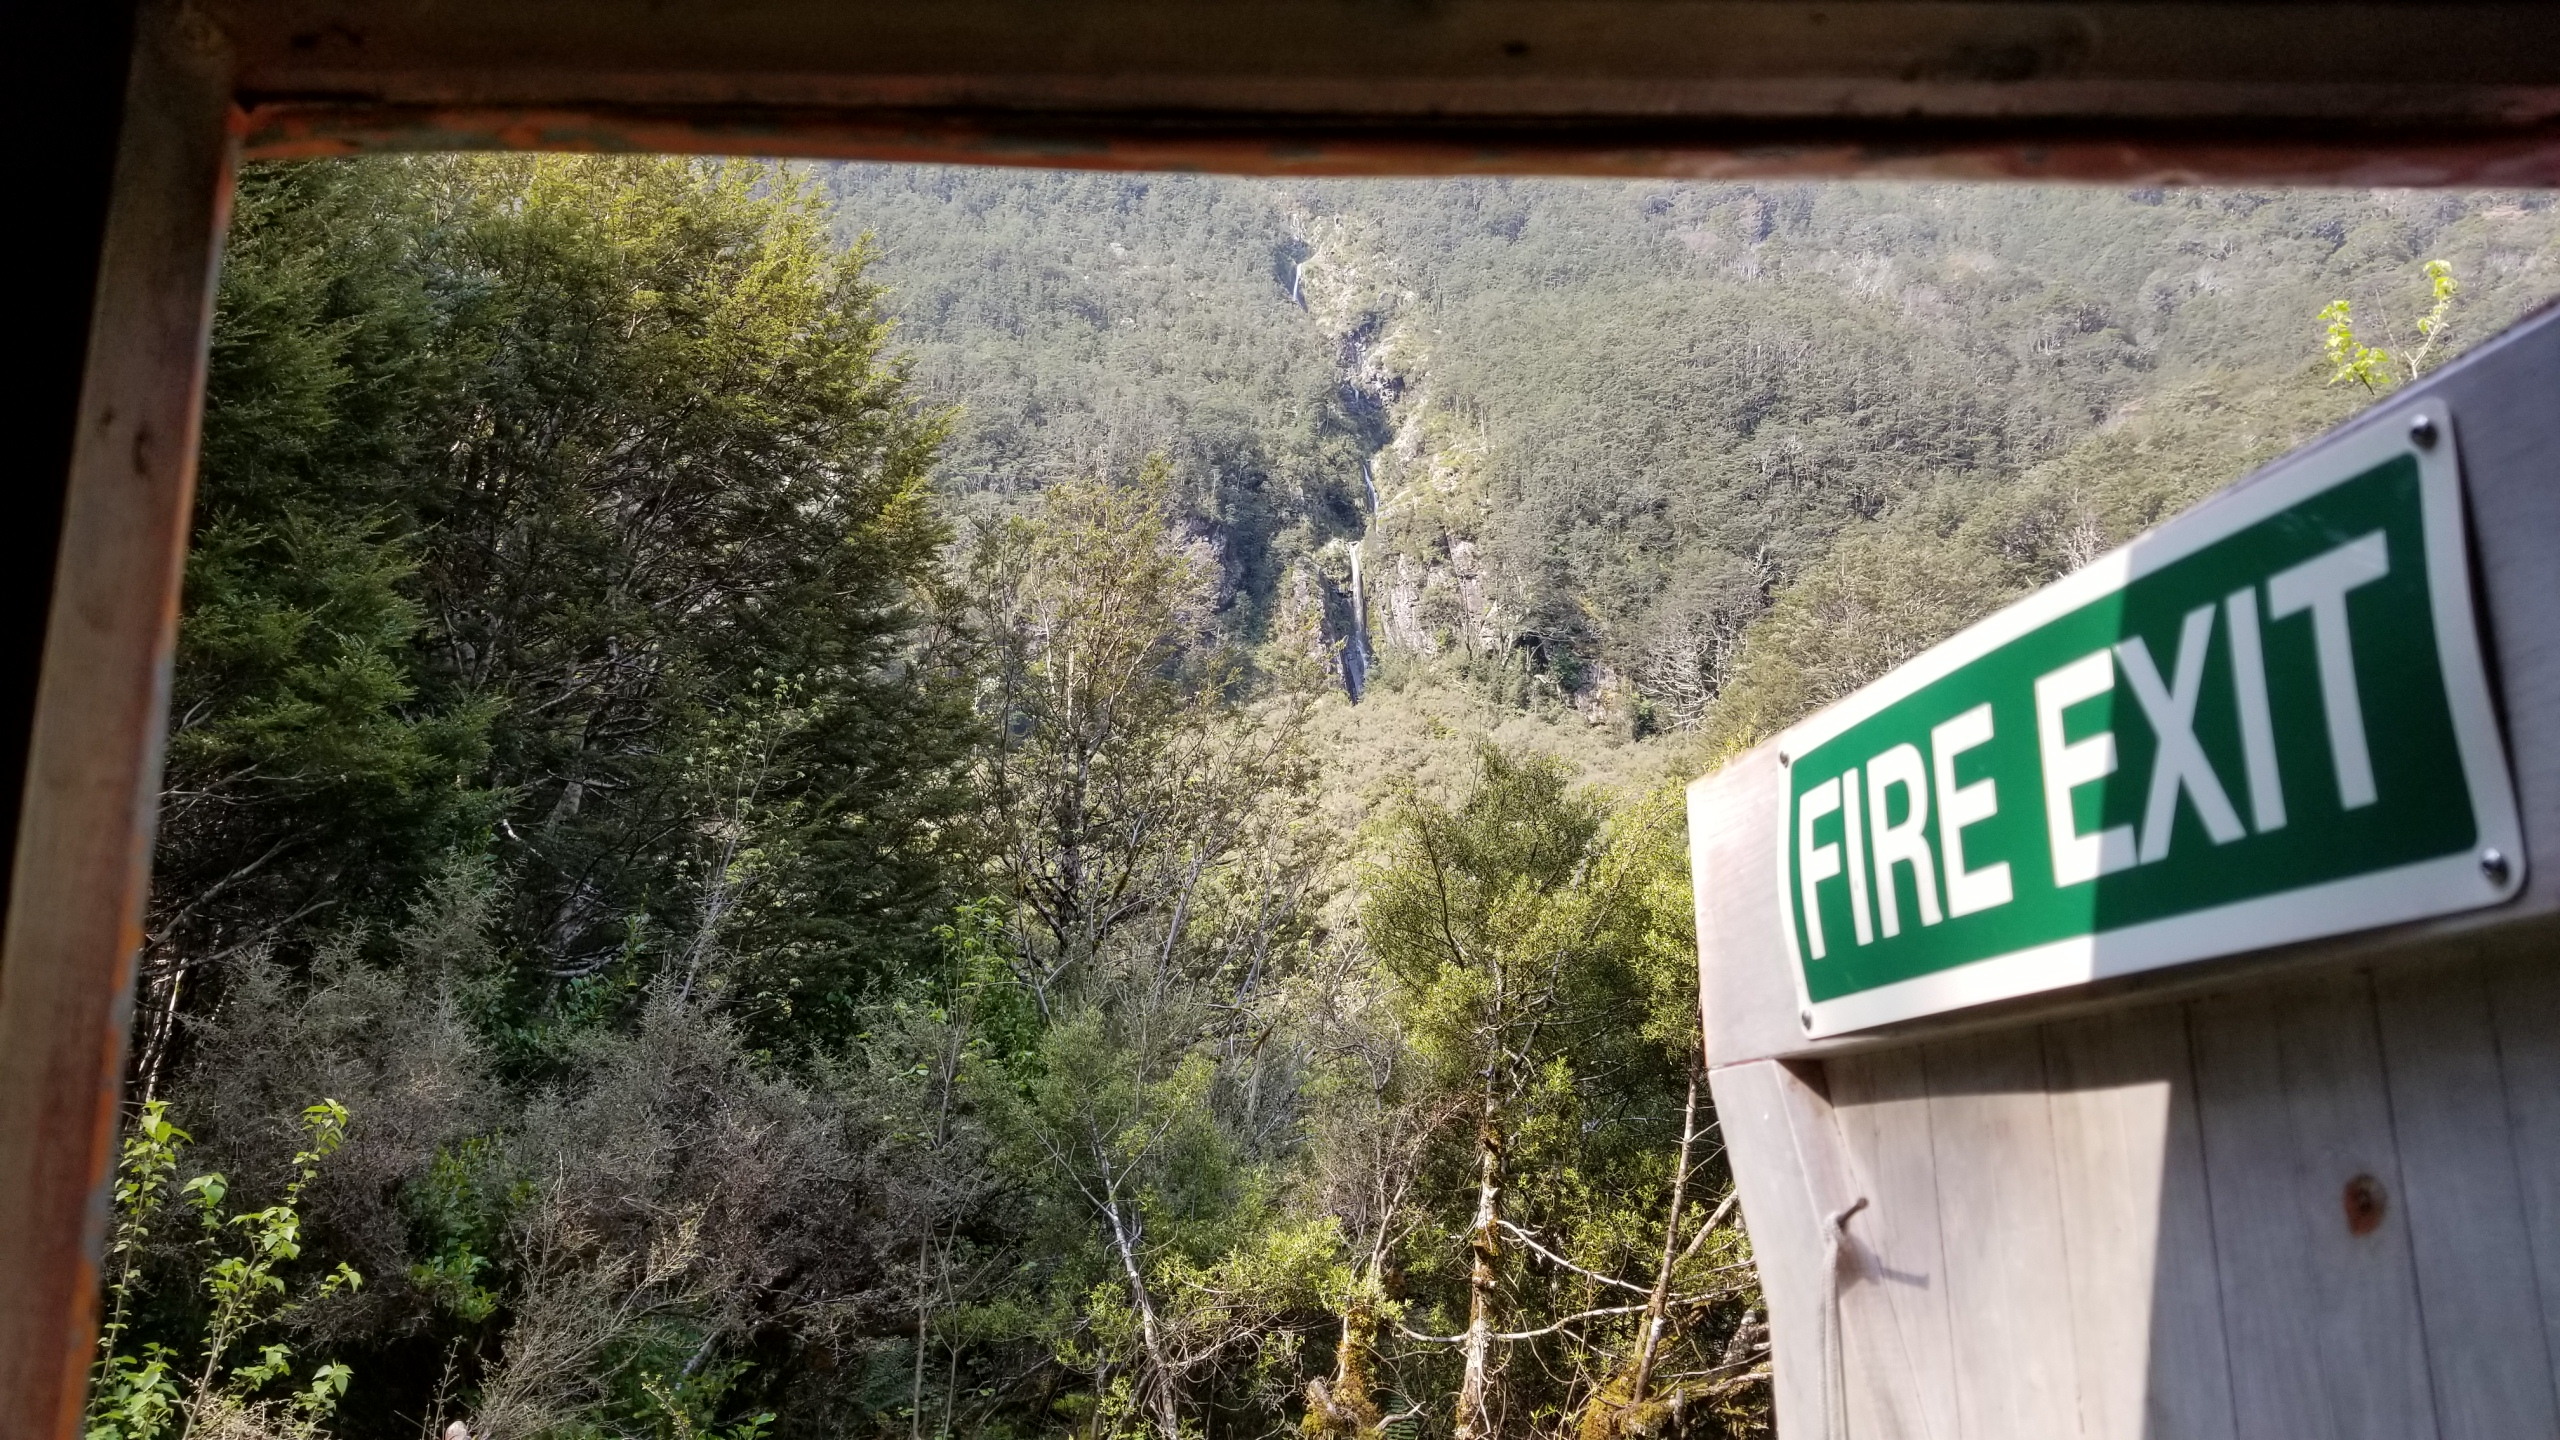
\includegraphics[width=8cm]{LucretiaBivReport23Nov2019Photo8}
   \caption{View from the door}
   \label{LB08}
\end{center}
\end{minipage}
\end{figure}

\section{Estimated cost of materials}

Based on the cost of renovating Lake Man Biv, it is estimated that this would cost about \$8000 ($\pm$ \$1000)

\begin{flushright}
Peter Alspach, Robyn Ritchie \& Brett Sandford\\
paalspach@gmail.com
\end{flushright}

\end{document}
